\section{Multithreading and multiprocessing in Python}

\subsection{Introduction and some clarifications}

The fundamental question of this section is: \textbf{How do we actually implement parallelism in Python?} 

Before answering, here's an important consideration.

The term \textit{program} might sometimes be used in an improper way\footnote{By that I mean that I've surely used it improperly as a synonym of process and I will probably continue to do so in the next sections.}. Technically a program is a \textit{passive} entity, typically a file stored on disk, e.g. your \texttt{.py} files. It contains the instructions but does not consume CPU resources until executed. 

Also, do not mix up the definition of a thread and that of a process: a process is an independent instance of a program that is executed by the operating system. \textit{Each process runs in its own memory space and has its own resources}, which means it does not share memory directly with other processes. Instead, threads share the same memory space and you can think of them as (the smallest) parts of the same process! 

\begin{center}
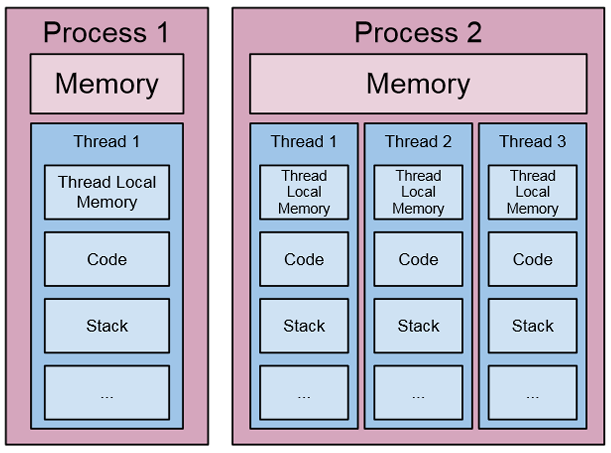
\includegraphics[width=0.5\textwidth]{figuresP/lesson_parallel_2A_pag_3.png}
\end{center}

Threads and processes are the fundamental blocks used to implement parallel programming in Python. 

A process could open another process during its execution (for example, if you run a Python program your code might launch an image editor) and the OS will have to assign resources and memory space to it accordingly. These processes don't "talk" to each other (unless you explicitly make them), which means for example that they don't share the same variables and functions. That makes them relatively less prone to some of the problems that we will soon talk about. They run independently and you can parallelize them with a multiprocessor. 

Threads are different. Parallelism happens when your code is written in a way that different operations can be completed simultaneously within the same memory space. That is riskier, but also much faster and lighter from the OS perspective, since it doesn't have to reassign anything. The term \textbf{Multithreading} refers to the simultaneous execution of different threads. 

\subsection{What not to do and how not to do it}
Parallel or concurrent execution (not only in Python) is very vulnerable to the following problems:
\begin{itemize}
    \item[-] \textbf{Starvation}: A task is constantly denied the necessary resources, so it can never finish ($\equiv$ it starves).
    \item[-] \textbf{Deadlock}: Two or more tasks wait cyclically for each other, causing a stall. 
    \begin{center}
        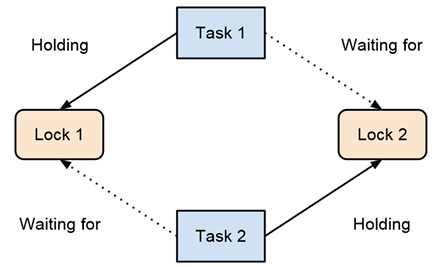
\includegraphics[width=0.35\textwidth]{figuresP/lesson_parallel_2A_pag_4.png}
    \end{center}
    \item[-] \textbf{Race condition}: A task that depends on the order of execution of the various threads or processes can produce wrongful results if such order is not respected. This is relevant for concurrency.
    \item[-] \textbf{Data corruption}: If two or more tasks try to work on the same memory location at the same time, the data you're working on can become corrupted during execution.
\end{itemize}
You need your program to be \textbf{thread-safe}, which means that it can be safely executed in a multithreaded environment without causing unexpected behaviour or errors, even when accessed by multiple threads simultaneously. Of course, that's going to take some careful programming, but fortunately there are some mechanisms that can help you avoid thread conflict.

For the most part, these are OS features that reserve the use of resources through synchronization primitives. For example, the \textbf{Mutex} is a locking mechanism: the first thread to require access to a certain memory location will be assigned a mutex token, it will access the memory and lock it so no other thread can interfere. Then the token passes onto the next thread and so on. The \textbf{Semaphore} system is a signalling mechanism that is just a generalization of the Mutex. A manager issues the ISR (Interrupt Signal Routing) and activates specific threads to avoid any conflict. \footnote{These mechanisms act on \textit{atomic operations}, at the lower level of the computer "brain".}

\subsection{The Global Interpreter Lock (GIL)}
Python implements a very simple thread-safe mechanism: the \textbf{Global Interpreter Lock (GIL)}. In order to prevent conflicts, only one statement in one thread is executed at a time (single-threading). In other words, the GIL seems to prevent multithreading, but don't worry: it can be deactivated. As of recent developments (e.g. Python 3.13+), there are ongoing efforts to make the GIL optional, but it remains a fundamental hurdle in standard environments.

Look at the following figure: there is a global lock that the current thread holds to safely access Python objects. Because only one thread can acquire Python Objects/C API, the interpreter regularly releases and reacquires the lock every 100 bytecodes of instructions. The frequency at which the interpreter checks for thread switching is controlled by the \texttt{sys.setcheckinterval()} function.

\begin{center}
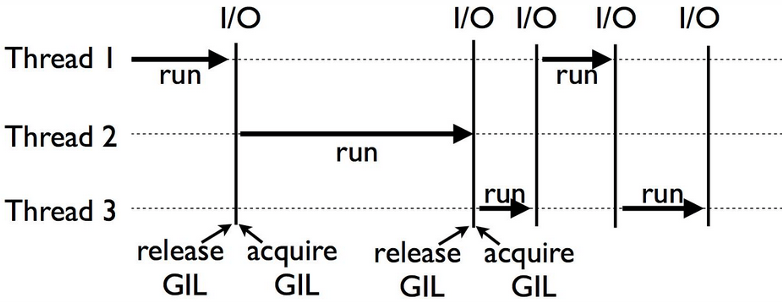
\includegraphics[width=0.6\textwidth]{figuresP/lesson_parallel_2A_pag_9.png}
\end{center}

There is only one exception to the global lock timing interval: the lock is released by a thread in case of an I/O operation, during which other threads can work concurrently. 

\begin{center}
    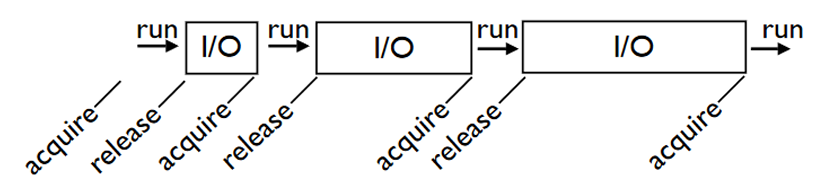
\includegraphics[width=0.6\textwidth]{figuresP/lesson_parallel_2A_pag_10.png}
\end{center}

It is important to note that, because of the GIL, CPU-bound applications won't be helped by threads. In Python, it is recommended to either use processes, or create a mixture of processes and threads. For this reason, \textit{Python is not the best language to use for parallelism}. So, what can we do? Python offers many libraries that provide wrappers for C functions. In other words, their classes and functions "steal" from the C language in order to let you work with parallelism.

Here's a short recap:

Pros and cons of processes:
\begin{itemize}
    \item[-] Can execute code simultaneously in the same Python program
    \item[-] Have separated memory space $\rightarrow$ less risky but difficult to communicate between them
    \item[-] Take advantage of multiple cores and CPUs
    \item[-] Avoid GIL limitations
    \item[-] Have relatively high overhead (opening and closing processes takes more time)
    \item[-] Child processes are killable
    \item[-] Model not adaptable to parallelism, better for concurrency
\end{itemize}

Pros and cons of threads:
\begin{itemize}
    \item[-] Use a shared memory $\rightarrow$ more risky (not in Python due to the GIL) but easier communication
    \item[-] Lightweight
    \item[-] Have very small overhead
    \item[-] Great option for I/O bound applications
    \item[-] Subject to GIL (although there are workarounds)
    \item[-] Not killable
    \item[-] Perfect for parallelism
\end{itemize}
So you should use\dots
\begin{itemize}
    \item[-] \dots\textit{processes} to speed up Python operations that are CPU intensive because they benefit from multiple cores and avoid the GIL.
    \item[-] \dots\textit{threads} for I/O tasks or tasks involving external systems because threads can combine their work more efficiently.
\end{itemize}

In the next sections we will (finally!) face some hands-on examples of parallel and concurrent computing in Python. You must learn how to use threads and processes, so we suggest you play along and write your own code. Also, during the in-person classes, these examples might have been analysed and explained a little more thoroughly than here, but if you've come this far you should have all the basics to understand what these new functions and classes do.

\subsection{Basics of multiprocessing in Python}

First of all, the basic modules needed to work with these mechanisms are \texttt{multiprocessing} and \texttt{threading}, so be sure you have them installed (they should already have been installed with your version of Python). The module \texttt{concurrent} (Python > 3.2) is an abstraction of multiprocessing and multithreading to simplify some functions.

Start by running \texttt{ps} on your Linux terminal. That will show all of your active processes:
\begin{verbatim}
lorenzo02@LAPTOP-AE9I3LPP:~/lezioni_computing_methods/parallel_python$ ps
    PID TTY          TIME CMD
    390 pts/0    00:00:00 bash
   9722 pts/0    00:00:00 ps
\end{verbatim}
With \texttt{ps -aux} you will be shown even the "hidden" processes (see documentation for more). 

\subsubsection{- First simple example: \texttt{Process}, \texttt{.start()}, \texttt{.join()}}
Take a look at the code below. The \texttt{Process} class from the \texttt{multiprocessing} module lets you easily manage processes in your code. The \texttt{.start()} method starts the execution of the child process (this is when the OS allocates memory space and resources for \texttt{p}). The \texttt{.join()} method tells the main process to wait for \texttt{p} to finish before continuing with its execution.

\begin{Verbatim}[label=\makebox{\url{https://github.com/lucabaldini/cmepda/tree/master/slides/latex/snippets/hello_multiprocessing.py}},commandchars=\\\{\}]
\PY{k}{from} \PY{n+nn}{multiprocessing} \PY{k}{import} \PY{n}{Process}

\PY{c+c1}{\# Defining a simple function...}
\PY{k}{def} \PY{n+nf}{f}\PY{p}{(}\PY{n}{name}\PY{p}{)}\PY{p}{:}
    \PY{n+nb}{print}\PY{p}{(}\PY{l+s+s1}{\PYZsq{}}\PY{l+s+s1}{Hello }\PY{l+s+s1}{\PYZsq{}}\PY{o}{+}\PY{n}{name}\PY{p}{)}

\PY{c+c1}{\# The function is execued in a child process,}
\PY{c+c1}{\# different than the one that was created by the HelloWorld.py program.}
\PY{k}{if} \PY{n}{\_\_name\_\_}\PY{o}{==}\PY{l+s+s2}{\PYZdq{}}\PY{l+s+s2}{\_\_main\_\_}\PY{l+s+s2}{\PYZdq{}}\PY{p}{:}
    \PY{n}{p} \PY{o}{=} \PY{n}{Process}\PY{p}{(}\PY{n}{target}\PY{o}{=}\PY{n}{f}\PY{p}{,} \PY{n}{args}\PY{o}{=}\PY{p}{(}\PY{l+s+s1}{\PYZsq{}}\PY{l+s+s1}{World}\PY{l+s+s1}{\PYZsq{}}\PY{p}{,}\PY{p}{)}\PY{p}{)}
    \PY{n}{p}\PY{o}{.}\PY{n}{start}\PY{p}{(}\PY{p}{)}
    \PY{n}{p}\PY{o}{.}\PY{n}{join}\PY{p}{(}\PY{p}{)}

[Output]
Hello World
\end{Verbatim}

\subsubsection{- Father and Sons}

If you run \texttt{ps} in your terminal, you will find that each process has a unique number called PID. In Python \texttt{os.getpid()} returns the PID of the current process, while \texttt{os.getppid()} executed in a secondary process (the child) returns the PID of the main one (the father). Pay attention to the PID numbers in the following example, which generates a tree of processes just like the one in the figure (PID numbers may vary):

\begin{Verbatim}[label=\makebox{\url{https://github.com/lucabaldini/cmepda/tree/master/slides/latex/snippets/FatherAndSons.py}},commandchars=\\\{\}]
\PY{k}{from} \PY{n+nn}{multiprocessing} \PY{k}{import} \PY{n}{Process}
\PY{k}{import} \PY{n+nn}{os}
\PY{k}{def} \PY{n+nf}{f0}\PY{p}{(}\PY{n}{name}\PY{p}{)}\PY{p}{:}
    \PY{n+nb}{print}\PY{p}{(}\PY{p}{)}
    \PY{n+nb}{print}\PY{p}{(}\PY{l+s+s2}{\PYZdq{}}\PY{l+s+s2}{\PYZhy{}\PYZhy{}\PYZhy{}\PYZhy{}\PYZgt{} function }\PY{l+s+s2}{\PYZdq{}}\PY{o}{+}\PY{n}{name}\PY{p}{)}
    \PY{n+nb}{print} \PY{p}{(}\PY{l+s+s2}{\PYZdq{}}\PY{l+s+s2}{I am still the main process with ID }\PY{l+s+s2}{\PYZdq{}}
           \PY{o}{+}\PY{n+nb}{str}\PY{p}{(}\PY{n}{os}\PY{o}{.}\PY{n}{getpid}\PY{p}{(}\PY{p}{)}\PY{p}{)}\PY{o}{+}\PY{l+s+s2}{\PYZdq{}}\PY{l+s+s2}{ my father is ID:}\PY{l+s+s2}{\PYZdq{}}\PY{o}{+}\PY{n+nb}{str}\PY{p}{(}\PY{n}{os}\PY{o}{.}\PY{n}{getppid}\PY{p}{(}\PY{p}{)}\PY{p}{)}\PY{p}{)}

\PY{k}{def} \PY{n+nf}{f1}\PY{p}{(}\PY{n}{name}\PY{p}{)}\PY{p}{:}
    \PY{n+nb}{print}\PY{p}{(}\PY{p}{)}
    \PY{n+nb}{print}\PY{p}{(}\PY{l+s+s2}{\PYZdq{}}\PY{l+s+s2}{\PYZhy{}\PYZhy{}\PYZhy{}\PYZhy{}\PYZgt{} function }\PY{l+s+s2}{\PYZdq{}}\PY{o}{+}\PY{n}{name}\PY{p}{)}
    \PY{n+nb}{print} \PY{p}{(}\PY{l+s+s2}{\PYZdq{}}\PY{l+s+s2}{I am the first sub\PYZhy{}process with ID }\PY{l+s+s2}{\PYZdq{}}
           \PY{o}{+}\PY{n+nb}{str}\PY{p}{(}\PY{n}{os}\PY{o}{.}\PY{n}{getpid}\PY{p}{(}\PY{p}{)}\PY{p}{)}\PY{o}{+}\PY{l+s+s2}{\PYZdq{}}\PY{l+s+s2}{ my father is ID:}\PY{l+s+s2}{\PYZdq{}}\PY{o}{+}\PY{n+nb}{str}\PY{p}{(}\PY{n}{os}\PY{o}{.}\PY{n}{getppid}\PY{p}{(}\PY{p}{)}\PY{p}{)}\PY{p}{)}
    \PY{n}{f2}\PY{p}{(}\PY{l+s+s1}{\PYZsq{}}\PY{l+s+s1}{two}\PY{l+s+s1}{\PYZsq{}}\PY{p}{)}


\PY{k}{def} \PY{n+nf}{f2}\PY{p}{(}\PY{n}{name}\PY{p}{)}\PY{p}{:}
    \PY{n+nb}{print}\PY{p}{(}\PY{p}{)}
    \PY{n+nb}{print}\PY{p}{(}\PY{l+s+s2}{\PYZdq{}}\PY{l+s+s2}{\PYZhy{}\PYZhy{}\PYZhy{}\PYZhy{}\PYZgt{} function }\PY{l+s+s2}{\PYZdq{}}\PY{o}{+}\PY{n}{name}\PY{p}{)}
    \PY{n+nb}{print} \PY{p}{(}\PY{l+s+s2}{\PYZdq{}}\PY{l+s+s2}{I am still the first sub\PYZhy{}process with ID }\PY{l+s+s2}{\PYZdq{}}
           \PY{o}{+}\PY{n+nb}{str}\PY{p}{(}\PY{n}{os}\PY{o}{.}\PY{n}{getpid}\PY{p}{(}\PY{p}{)}\PY{p}{)}\PY{o}{+}\PY{l+s+s2}{\PYZdq{}}\PY{l+s+s2}{ my father is ID:}\PY{l+s+s2}{\PYZdq{}}\PY{o}{+}\PY{n+nb}{str}\PY{p}{(}\PY{n}{os}\PY{o}{.}\PY{n}{getppid}\PY{p}{(}\PY{p}{)}\PY{p}{)}\PY{p}{)}
    \PY{n+nb}{print}\PY{p}{(}\PY{l+s+s2}{\PYZdq{}}\PY{l+s+s2}{This is the end!}\PY{l+s+s2}{\PYZdq{}}\PY{p}{)}

\PY{c+c1}{\#MAIN}
\PY{k}{if} \PY{n}{\_\_name\_\_}\PY{o}{==}\PY{l+s+s2}{\PYZdq{}}\PY{l+s+s2}{\_\_main\_\_}\PY{l+s+s2}{\PYZdq{}}\PY{p}{:}
    \PY{n+nb}{print} \PY{p}{(}\PY{l+s+s2}{\PYZdq{}}\PY{l+s+s2}{I am the main process with ID: }\PY{l+s+s2}{\PYZdq{}}\PY{o}{+}\PY{n+nb}{str}\PY{p}{(}\PY{n}{os}\PY{o}{.}\PY{n}{getpid}\PY{p}{(}\PY{p}{)}\PY{p}{)}\PY{p}{)}
    \PY{n}{f0}\PY{p}{(}\PY{l+s+s1}{\PYZsq{}}\PY{l+s+s1}{zero}\PY{l+s+s1}{\PYZsq{}}\PY{p}{)}
    \PY{n}{p} \PY{o}{=} \PY{n}{Process}\PY{p}{(}\PY{n}{target}\PY{o}{=}\PY{n}{f1}\PY{p}{,} \PY{n}{args}\PY{o}{=}\PY{p}{(}\PY{l+s+s1}{\PYZsq{}}\PY{l+s+s1}{one}\PY{l+s+s1}{\PYZsq{}}\PY{p}{,}\PY{p}{)}\PY{p}{)}
    \PY{n}{p}\PY{o}{.}\PY{n}{start}\PY{p}{(}\PY{p}{)}
    \PY{n}{p}\PY{o}{.}\PY{n}{join}\PY{p}{(}\PY{p}{)}

[Output]
I am the main process with ID:2420

-----> function zero
I am still the main process with ID 3384 my father is ID:2420

-----> function one
I am the first sub-process with ID 3385 my father is ID:3384

-----> function two
I am still the first sub-process with ID 3385 my father is ID:3384
This is the end!
\end{Verbatim}

\begin{center}
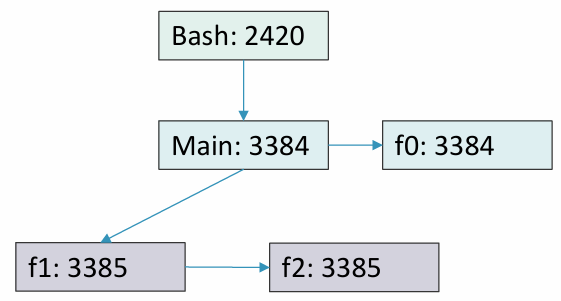
\includegraphics[width=0.4\textwidth]{figuresP/lesson_parallel_2B_pag_8}
\end{center}

Note: You might not be familiar with the \texttt{if \_\_name\_\_ == "\_\_main\_\_"} line, but it's very common in Python programming. It's there only so that if you import that module you won't automatically run the code under the \texttt{if} statement. The name of your process is \texttt{"\_\_main\_\_"} only if you run that program directly. 

\subsubsection{- Function on 4 processes: the \texttt{Queue}}

What if you wanted to run the same function on 4 different processes? You need to use a \texttt{Queue}.

The \texttt{Queue} class lets you create and manage a queue of processes, and it's the "letterbox" that lets such processes send variables to the main one: \texttt{Queue.put()} inserts an object in the queue while \texttt{Queue.get()} extracts an object from it. Here's how to use them:

\begin{Verbatim}[label=\makebox{\url{https://github.com/lucabaldini/cmepda/tree/master/slides/latex/snippets/multiprocessing_queue.py}},commandchars=\\\{\}]
\PY{k}{import} \PY{n+nn}{multiprocessing} \PY{k}{as} \PY{n+nn}{mp}

\PY{c+c1}{\# Define an example function}
\PY{k}{def} \PY{n+nf}{Hello}\PY{p}{(}\PY{n}{pos}\PY{p}{,}\PY{n}{name}\PY{p}{)}\PY{p}{:}
    \PY{n}{msg}\PY{o}{=}\PY{l+s+s2}{\PYZdq{}}\PY{l+s+s2}{Hello }\PY{l+s+s2}{\PYZdq{}}\PY{o}{+}\PY{n}{name}
    \PY{n}{output}\PY{o}{.}\PY{n}{put}\PY{p}{(}\PY{p}{(}\PY{n}{pos}\PY{p}{,} \PY{n}{msg}\PY{p}{)}\PY{p}{)}

\PY{k}{if} \PY{n}{\_\_name\_\_}\PY{o}{==}\PY{l+s+s2}{\PYZdq{}}\PY{l+s+s2}{\_\_main\_\_}\PY{l+s+s2}{\PYZdq{}}\PY{p}{:}
    \PY{c+c1}{\# Define an output queue}
    \PY{n}{output} \PY{o}{=} \PY{n}{mp}\PY{o}{.}\PY{n}{Queue}\PY{p}{(}\PY{p}{)}
    \PY{c+c1}{\# Setup a list of processes that we want to run}
    \PY{n}{processes} \PY{o}{=} \PY{p}{[}\PY{n}{mp}\PY{o}{.}\PY{n}{Process}\PY{p}{(}\PY{n}{target}\PY{o}{=}\PY{n}{Hello}\PY{p}{,} \PY{n}{args}\PY{o}{=}\PY{p}{(}\PY{n}{x}\PY{p}{,} \PY{l+s+s2}{\PYZdq{}}\PY{l+s+s2}{Gianluca}\PY{l+s+s2}{\PYZdq{}}\PY{p}{)}\PY{p}{)} \PY{k}{for} \PY{n}{x} \PY{k}{in} \PY{n+nb}{range}\PY{p}{(}\PY{l+m+mi}{4}\PY{p}{)}\PY{p}{]}
    
    \PY{c+c1}{\# Run processes}
    \PY{k}{for} \PY{n}{p} \PY{k}{in} \PY{n}{processes}\PY{p}{:}
        \PY{n}{p}\PY{o}{.}\PY{n}{start}\PY{p}{(}\PY{p}{)}

    \PY{c+c1}{\# Exit the completed processes}
    \PY{k}{for} \PY{n}{p} \PY{k}{in} \PY{n}{processes}\PY{p}{:}
        \PY{n}{p}\PY{o}{.}\PY{n}{join}\PY{p}{(}\PY{p}{)}
            
    \PY{c+c1}{\# Get process results from the output queue}
    \PY{n}{results} \PY{o}{=} \PY{p}{[}\PY{n}{output}\PY{o}{.}\PY{n}{get}\PY{p}{(}\PY{p}{)} \PY{k}{for} \PY{n}{p} \PY{k}{in} \PY{n}{processes}\PY{p}{]}
    \PY{n+nb}{print}\PY{p}{(}\PY{n}{results}\PY{p}{)}

[Output]
[(0, 'Hello Gianluca'), (1, 'Hello Gianluca'), (2, 'Hello Gianluca'), (3, 'Hello Gianluca')]
\end{Verbatim}

\subsubsection{- Distributing your work: the \texttt{Pool}}

Using the \texttt{Pool} class, you can define a certain number of processes that will run on different cores (if your computer has more than one). Take a look at the code below:
\begin{itemize}
    \item[-] \texttt{Pool.map()} stops the execution of the main program and runs your processes (\textit{synchronous run});
    \item[-] \texttt{Pool.map\_async()} runs your processes without stopping the main one. That's why in the second example you need a \texttt{timeout} before retrieving the results: you have to make sure that your processes are done (\textit{asynchronous run}). 
\end{itemize}
Pay attention to the PID numbers: can you tell in what order and by which process the 6 operations were executed? 

See also the documentation for  \texttt{Pool.apply()} and \texttt{Pool.apply\_async()}, which have similar effects. 

Here is an example demonstrating the synchronous \texttt{Pool.map()}:

\begin{Verbatim}[label=\makebox{\url{https://github.com/lucabaldini/cmepda/tree/master/slides/latex/snippets/multiprocessing_pool_map.py}},commandchars=\\\{\}]
\PY{k}{import} \PY{n+nn}{multiprocessing} \PY{k}{as} \PY{n+nn}{mp}
\PY{k}{import} \PY{n+nn}{time}
\PY{k}{import} \PY{n+nn}{os}

\PY{k}{def} \PY{n+nf}{cube}\PY{p}{(}\PY{n}{x}\PY{p}{)}\PY{p}{:}
    \PY{n+nb}{print} \PY{p}{(}\PY{n+nb}{str}\PY{p}{(}\PY{n}{os}\PY{o}{.}\PY{n}{getpid}\PY{p}{(}\PY{p}{)}\PY{p}{)}\PY{o}{+}\PY{l+s+s2}{\PYZdq{}}\PY{l+s+s2}{ }\PY{l+s+s2}{\PYZdq{}}\PY{o}{+}\PY{n+nb}{str}\PY{p}{(}\PY{n}{os}\PY{o}{.}\PY{n}{getppid}\PY{p}{(}\PY{p}{)}\PY{p}{)}\PY{o}{+}\PY{l+s+s2}{\PYZdq{}}\PY{l+s+s2}{ }\PY{l+s+s2}{\PYZdq{}}\PY{o}{+}\PY{n+nb}{str}\PY{p}{(}\PY{n}{x}\PY{o}{**}\PY{l+m+mi}{3}\PY{p}{)}\PY{p}{)}
    \PY{k}{return} \PY{n}{x}\PY{o}{**}\PY{l+m+mi}{3}

\PY{k}{if} \PY{n}{\_\_name\_\_}\PY{o}{==}\PY{l+s+s2}{\PYZdq{}}\PY{l+s+s2}{\_\_main\_\_}\PY{l+s+s2}{\PYZdq{}}\PY{p}{:}
    \PY{c+c1}{\# Define a group of processes (\PYZdq{}workers\PYZdq{})}
    \PY{n}{pool} \PY{o}{=} \PY{n}{mp}\PY{o}{.}\PY{n}{Pool}\PY{p}{(}\PY{n}{processes}\PY{o}{=}\PY{l+m+mi}{4}\PY{p}{)}
    \PY{c+c1}{\# Make each worker do something (even if \# tasks \PYZgt{} \# workers)}
    \PY{n}{results} \PY{o}{=} \PY{n}{pool}\PY{o}{.}\PY{n}{map}\PY{p}{(}\PY{n}{cube}\PY{p}{,} \PY{n+nb}{range}\PY{p}{(}\PY{l+m+mi}{1}\PY{p}{,}\PY{l+m+mi}{7}\PY{p}{)}\PY{p}{)}
    \PY{c+c1}{\# Print the results}
    \PY{n+nb}{print}\PY{p}{(}\PY{n}{results}\PY{p}{)}

[Output]
17348 17346 8
17347 17346 1
17349 17346 27
17350 17346 64
17348 17346 125
17347 17346 216
[1, 8, 27, 64, 125, 216]
\end{Verbatim}
\bigskip
\hrulefill
\bigskip

And here is the asynchronous equivalent using \texttt{Pool.map\_async()}:

\begin{Verbatim}[label=\makebox{\url{https://github.com/lucabaldini/cmepda/tree/master/slides/latex/snippets/multiprocessing_map_async_timeout.py}},commandchars=\\\{\}]
\PY{k}{import} \PY{n+nn}{multiprocessing} \PY{k}{as} \PY{n+nn}{mp}
\PY{k}{import} \PY{n+nn}{os}

\PY{k}{def} \PY{n+nf}{cube}\PY{p}{(}\PY{n}{x}\PY{p}{)}\PY{p}{:}
    \PY{n+nb}{print} \PY{p}{(}\PY{n+nb}{str}\PY{p}{(}\PY{n}{os}\PY{o}{.}\PY{n}{getpid}\PY{p}{(}\PY{p}{)}\PY{p}{)}\PY{o}{+}\PY{l+s+s2}{\PYZdq{}}\PY{l+s+s2}{ }\PY{l+s+s2}{\PYZdq{}}\PY{o}{+}\PY{n+nb}{str}\PY{p}{(}\PY{n}{os}\PY{o}{.}\PY{n}{getppid}\PY{p}{(}\PY{p}{)}\PY{p}{)}\PY{o}{+}\PY{l+s+s2}{\PYZdq{}}\PY{l+s+s2}{ }\PY{l+s+s2}{\PYZdq{}}\PY{o}{+}\PY{n+nb}{str}\PY{p}{(}\PY{n}{x}\PY{o}{**}\PY{l+m+mi}{3}\PY{p}{)}\PY{p}{)}
    \PY{k}{return} \PY{n}{x}\PY{o}{**}\PY{l+m+mi}{3}

\PY{k}{if} \PY{n}{\_\_name\_\_}\PY{o}{==}\PY{l+s+s2}{\PYZdq{}}\PY{l+s+s2}{\_\_main\_\_}\PY{l+s+s2}{\PYZdq{}}\PY{p}{:}
    \PY{c+c1}{\# Define a group of processes (\PYZdq{}workers\PYZdq{})}
    \PY{n}{pool} \PY{o}{=} \PY{n}{mp}\PY{o}{.}\PY{n}{Pool}\PY{p}{(}\PY{n}{processes}\PY{o}{=}\PY{l+m+mi}{4}\PY{p}{)}
    \PY{c+c1}{\# Make each worker do something without interrupting the main process}
    \PY{n}{results} \PY{o}{=} \PY{n}{pool}\PY{o}{.}\PY{n}{map\_async}\PY{p}{(}\PY{n}{cube}\PY{p}{,} \PY{n+nb}{range}\PY{p}{(}\PY{l+m+mi}{1}\PY{p}{,}\PY{l+m+mi}{7}\PY{p}{)}\PY{p}{)}
    \PY{c+c1}{\# Print the results using a timeout to be sure results is full}
    \PY{n+nb}{print}\PY{p}{(}\PY{n}{results}\PY{o}{.}\PY{n}{get}\PY{p}{(}\PY{n}{timeout}\PY{o}{=}\PY{l+m+mi}{1}\PY{p}{)}\PY{p}{)}

[Output]
17428 17425 1
17429 17425 8
17428 17425 64
17428 17425 216
17431 17425 125
17430 17425 27
[1, 8, 27, 64, 125, 216]
\end{Verbatim}

Let's create a function with a "sleep" time using the \texttt{time} module to simulate a longer execution. Take a look at the two versions of the code. In the synchronous example, the time needed to execute the main process is about 6 seconds (since it has to wait for the child processes, 3 + 3 seconds) while in the asynchronous one the \texttt{elapsed\_time} is less than a second. Of course, the latter didn't actually run faster, but we closed the main process before the others had ended (in fact, the output seems truncated). In this case our function doesn't return anything, otherwise our \texttt{timeout} would have slowed the main process down. 

\begin{Verbatim}[label=\makebox{\url{https://github.com/lucabaldini/cmepda/tree/master/slides/latex/snippets/multiprocessing_pool_doingstuff.py}},commandchars=\\\{\}]
\PY{k}{import} \PY{n+nn}{multiprocessing} \PY{k}{as} \PY{n+nn}{mp}
\PY{k}{import} \PY{n+nn}{time}
\PY{k}{import} \PY{n+nn}{os}

\PY{k}{def} \PY{n+nf}{doingstuff}\PY{p}{(}\PY{n}{x}\PY{p}{)}\PY{p}{:}
    \PY{n+nb}{print} \PY{p}{(}\PY{l+s+s2}{\PYZdq{}}\PY{l+s+s2}{Process: }\PY{l+s+s2}{\PYZdq{}}\PY{o}{+}\PY{n+nb}{str}\PY{p}{(}\PY{n}{x}\PY{p}{)}\PY{o}{+}\PY{l+s+s2}{\PYZdq{}}\PY{l+s+s2}{ }\PY{l+s+s2}{\PYZdq{}}\PY{o}{+}\PY{n+nb}{str}\PY{p}{(}\PY{n}{os}\PY{o}{.}\PY{n}{getpid}\PY{p}{(}\PY{p}{)}\PY{p}{)}\PY{p}{)}
    \PY{c+c1}{\# Add a delay}
    \PY{n}{time}\PY{o}{.}\PY{n}{sleep}\PY{p}{(}\PY{l+m+mi}{3}\PY{p}{)}

\PY{k}{if} \PY{n}{\_\_name\_\_}\PY{o}{==}\PY{l+s+s2}{\PYZdq{}}\PY{l+s+s2}{\_\_main\_\_}\PY{l+s+s2}{\PYZdq{}}\PY{p}{:}
    \PY{c+c1}{\# Start the timer}
    \PY{n}{start}\PY{o}{=}\PY{n}{time}\PY{o}{.}\PY{n}{time}\PY{p}{(}\PY{p}{)}
    \PY{c+c1}{\# Define a group of processes (\PYZdq{}workers\PYZdq{})}
    \PY{n}{pool} \PY{o}{=} \PY{n}{mp}\PY{o}{.}\PY{n}{Pool}\PY{p}{(}\PY{n}{processes}\PY{o}{=}\PY{l+m+mi}{4}\PY{p}{)}
    \PY{c+c1}{\# Make each worker do something}
    \PY{n}{results} \PY{o}{=} \PY{n}{pool}\PY{o}{.}\PY{n}{map}\PY{p}{(}\PY{n}{doingstuff}\PY{p}{,} \PY{n+nb}{range}\PY{p}{(}\PY{l+m+mi}{1}\PY{p}{,}\PY{l+m+mi}{10}\PY{p}{)}\PY{p}{)}
    \PY{c+c1}{\# Stop the timer}
    \PY{n}{end}\PY{o}{=}\PY{n}{time}\PY{o}{.}\PY{n}{time}\PY{p}{(}\PY{p}{)}
    \PY{n+nb}{print}\PY{p}{(}\PY{l+s+s2}{\PYZdq{}}\PY{l+s+s2}{elapsed time: }\PY{l+s+s2}{\PYZdq{}}\PY{o}{+}\PY{n+nb}{str}\PY{p}{(}\PY{n}{end}\PY{o}{\PYZhy{}}\PY{n}{start}\PY{p}{)}\PY{p}{)}

[Output]
Process: 1 19112
Process: 2 19113
Process: 3 19114
Process: 4 19115
Process: 5 19112
Process: 6 19113
Process: 7 19114
Process: 8 19115
Process: 9 19113
elapsed time: 9.066443681716919
\end{Verbatim}
\bigskip
\hrulefill
\bigskip

\begin{Verbatim}[label=\makebox{\url{https://github.com/lucabaldini/cmepda/tree/master/slides/latex/snippets/multiprocessing_pool_doingstuff_async.py}},commandchars=\\\{\}]
\PY{k}{import} \PY{n+nn}{multiprocessing} \PY{k}{as} \PY{n+nn}{mp}
\PY{k}{import} \PY{n+nn}{time}
\PY{k}{import} \PY{n+nn}{os}

\PY{k}{def} \PY{n+nf}{doingstuff}\PY{p}{(}\PY{n}{x}\PY{p}{)}\PY{p}{:}
    \PY{n+nb}{print} \PY{p}{(}\PY{l+s+s2}{\PYZdq{}}\PY{l+s+s2}{Process: }\PY{l+s+s2}{\PYZdq{}}\PY{o}{+}\PY{n+nb}{str}\PY{p}{(}\PY{n}{x}\PY{p}{)}\PY{o}{+}\PY{l+s+s2}{\PYZdq{}}\PY{l+s+s2}{ }\PY{l+s+s2}{\PYZdq{}}\PY{o}{+}\PY{n+nb}{str}\PY{p}{(}\PY{n}{os}\PY{o}{.}\PY{n}{getpid}\PY{p}{(}\PY{p}{)}\PY{p}{)}\PY{p}{)}
    \PY{c+c1}{\# Add a delay}
    \PY{n}{time}\PY{o}{.}\PY{n}{sleep}\PY{p}{(}\PY{l+m+mi}{3}\PY{p}{)}

\PY{k}{if} \PY{n}{\_\_name\_\_}\PY{o}{==}\PY{l+s+s2}{\PYZdq{}}\PY{l+s+s2}{\_\_main\_\_}\PY{l+s+s2}{\PYZdq{}}\PY{p}{:}
    \PY{c+c1}{\# Start the timer}
    \PY{n}{start}\PY{o}{=}\PY{n}{time}\PY{o}{.}\PY{n}{time}\PY{p}{(}\PY{p}{)}
    \PY{c+c1}{\# Define a group of processes (\PYZdq{}workers\PYZdq{})}
    \PY{n}{pool} \PY{o}{=} \PY{n}{mp}\PY{o}{.}\PY{n}{Pool}\PY{p}{(}\PY{n}{processes}\PY{o}{=}\PY{l+m+mi}{4}\PY{p}{)}
    \PY{c+c1}{\# Make each worker do something}
    \PY{n}{results} \PY{o}{=} \PY{n}{pool}\PY{o}{.}\PY{n}{map\_async}\PY{p}{(}\PY{n}{doingstuff}\PY{p}{,} \PY{n+nb}{range}\PY{p}{(}\PY{l+m+mi}{1}\PY{p}{,}\PY{l+m+mi}{10}\PY{p}{)}\PY{p}{)}
    \PY{c+c1}{\# Stop the timer}
    \PY{n}{end}\PY{o}{=}\PY{n}{time}\PY{o}{.}\PY{n}{time}\PY{p}{(}\PY{p}{)}
    \PY{n+nb}{print}\PY{p}{(}\PY{l+s+s2}{\PYZdq{}}\PY{l+s+s2}{elapsed time: }\PY{l+s+s2}{\PYZdq{}}\PY{o}{+}\PY{n+nb}{str}\PY{p}{(}\PY{n}{end}\PY{o}{\PYZhy{}}\PY{n}{start}\PY{p}{)}\PY{p}{)}

[Output]
elapsed time: 0.028638362884521484
Process: 1 19211
Process: 2 19212
Process: 3 19213
Process: 4 19214
\end{Verbatim}

\subsection{Communicating processes in Python}

\subsubsection{- Shared memory}

In the following code a dangerous mechanism is shown: the main process and the child one seem to share a global variable, but the result is a disaster!

\begin{Verbatim}[label=\makebox{\url{https://github.com/lucabaldini/cmepda/tree/master/slides/latex/snippets/multiprocessing_global_scope.py}},commandchars=\\\{\}]
\PY{k}{import} \PY{n+nn}{multiprocessing}

\PY{c+c1}{\# Empty list with global scope}
\PY{n}{result} \PY{o}{=} \PY{p}{[}\PY{p}{]}

\PY{k}{def} \PY{n+nf}{square\_list}\PY{p}{(}\PY{n}{mylist}\PY{p}{)}\PY{p}{:}
        \PY{k}{global} \PY{n}{result}
        \PY{k}{for} \PY{n}{num} \PY{k}{in} \PY{n}{mylist}\PY{p}{:}
                \PY{n}{result}\PY{o}{.}\PY{n}{append}\PY{p}{(}\PY{n}{num} \PY{o}{*} \PY{n}{num}\PY{p}{)}
        \PY{c+c1}{\# Print result list from the function}
        \PY{n+nb}{print}\PY{p}{(}\PY{l+s+s2}{\PYZdq{}}\PY{l+s+s2}{Result(in process p1): }\PY{l+s+s2}{\PYZdq{}}\PY{o}{+}\PY{n+nb}{str}\PY{p}{(}\PY{n}{result}\PY{p}{)}\PY{p}{)}

\PY{k}{if} \PY{n}{\_\_name\_\_}\PY{o}{==}\PY{l+s+s2}{\PYZdq{}}\PY{l+s+s2}{\_\_main\_\_}\PY{l+s+s2}{\PYZdq{}}\PY{p}{:}
    \PY{c+c1}{\# Input list}
    \PY{n}{mylist} \PY{o}{=} \PY{p}{[}\PY{l+m+mi}{1}\PY{p}{,}\PY{l+m+mi}{2}\PY{p}{,}\PY{l+m+mi}{3}\PY{p}{,}\PY{l+m+mi}{4}\PY{p}{]}
    \PY{c+c1}{\# Creating the new process}
    \PY{n}{p1} \PY{o}{=} \PY{n}{multiprocessing}\PY{o}{.}\PY{n}{Process}\PY{p}{(}\PY{n}{target}\PY{o}{=}\PY{n}{square\_list}\PY{p}{,} \PY{n}{args}\PY{o}{=}\PY{p}{(}\PY{n}{mylist}\PY{p}{,}\PY{p}{)}\PY{p}{)}
    \PY{n}{p1}\PY{o}{.}\PY{n}{start}\PY{p}{(}\PY{p}{)}
    \PY{n}{p1}\PY{o}{.}\PY{n}{join}\PY{p}{(}\PY{p}{)}
    \PY{c+c1}{\# Print global result list}
    \PY{n+nb}{print}\PY{p}{(}\PY{l+s+s2}{\PYZdq{}}\PY{l+s+s2}{Result(in main program): }\PY{l+s+s2}{\PYZdq{}}\PY{o}{+}\PY{n+nb}{str}\PY{p}{(}\PY{n}{result}\PY{p}{)}\PY{p}{)}

[Output]
Result(in process p1): [1, 4, 9, 16]
Result(in main program): []
\end{Verbatim}

Always remember: different processes have different memory spaces, so the \texttt{result} variable is not modified in the main process. 

In order to correctly work out this task, you can create a shared memory space between the two processes. Here this is done using the \texttt{Array} and the \texttt{Value} classes, which respectively create a "location" (we will see that the correct term is \textit{pointer}) in the shared memory for an array and for a value. In this example, we fill these locations with the results of our processes. 

\begin{center}
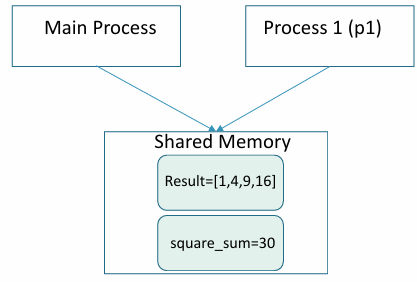
\includegraphics[width=0.4\textwidth]{figuresP/lesson_parallel_2B_pag_12}
\end{center}

\begin{Verbatim}[label=\makebox{\url{https://github.com/lucabaldini/cmepda/tree/master/slides/latex/snippets/multiprocessing_shared_memory.py}},commandchars=\\\{\}]
\PY{k}{import} \PY{n+nn}{multiprocessing}

\PY{k}{def} \PY{n+nf}{square\_list}\PY{p}{(}\PY{n}{mylist}\PY{p}{,} \PY{n}{result}\PY{p}{,} \PY{n}{square\_sum}\PY{p}{)}\PY{p}{:}
    \PY{k}{for} \PY{n}{idx}\PY{p}{,} \PY{n}{num} \PY{k}{in} \PY{n+nb}{enumerate}\PY{p}{(}\PY{n}{mylist}\PY{p}{)}\PY{p}{:}
        \PY{n}{result}\PY{p}{[}\PY{n}{idx}\PY{p}{]} \PY{o}{=} \PY{n}{num} \PY{o}{*} \PY{n}{num}
    \PY{c+c1}{\# Square\_sum value}
    \PY{n}{square\_sum}\PY{o}{.}\PY{n}{value} \PY{o}{=} \PY{n+nb}{sum}\PY{p}{(}\PY{n}{result}\PY{p}{)}
    \PY{c+c1}{\# Print result Array}
    \PY{n+nb}{print}\PY{p}{(}\PY{l+s+s2}{\PYZdq{}}\PY{l+s+s2}{Result(in process p1): }\PY{l+s+s2}{\PYZdq{}}\PY{o}{+}\PY{n+nb}{str}\PY{p}{(}\PY{n}{result}\PY{p}{[}\PY{p}{:}\PY{p}{]}\PY{p}{)}\PY{p}{)}
    \PY{c+c1}{\# Print square\_sum Value}
    \PY{n+nb}{print}\PY{p}{(}\PY{l+s+s2}{\PYZdq{}}\PY{l+s+s2}{Sum of squares(in process p1): }\PY{l+s+s2}{\PYZdq{}}\PY{o}{+}\PY{n+nb}{str}\PY{p}{(}\PY{n}{square\_sum}\PY{o}{.}\PY{n}{value}\PY{p}{)}\PY{p}{)}

\PY{k}{if} \PY{n}{\_\_name\_\_}\PY{o}{==}\PY{l+s+s2}{\PYZdq{}}\PY{l+s+s2}{\_\_main\_\_}\PY{l+s+s2}{\PYZdq{}}\PY{p}{:}
    \PY{c+c1}{\# Input list}
    \PY{n}{mylist} \PY{o}{=} \PY{p}{[}\PY{l+m+mi}{1}\PY{p}{,}\PY{l+m+mi}{2}\PY{p}{,}\PY{l+m+mi}{3}\PY{p}{,}\PY{l+m+mi}{4}\PY{p}{]}
    \PY{c+c1}{\# Creating Array of int data type with space for 4 integers}
    \PY{n}{result} \PY{o}{=} \PY{n}{multiprocessing}\PY{o}{.}\PY{n}{Array}\PY{p}{(}\PY{l+s+s1}{\PYZsq{}}\PY{l+s+s1}{i}\PY{l+s+s1}{\PYZsq{}}\PY{p}{,} \PY{l+m+mi}{4}\PY{p}{)}
    \PY{c+c1}{\# Creating Value of int data type}
    \PY{n}{square\_sum} \PY{o}{=} \PY{n}{multiprocessing}\PY{o}{.}\PY{n}{Value}\PY{p}{(}\PY{l+s+s1}{\PYZsq{}}\PY{l+s+s1}{i}\PY{l+s+s1}{\PYZsq{}}\PY{p}{)}

    \PY{c+c1}{\# Creating the new process}
    \PY{n}{p1} \PY{o}{=} \PY{n}{multiprocessing}\PY{o}{.}\PY{n}{Process}\PY{p}{(}\PY{n}{target}\PY{o}{=}\PY{n}{square\_list}\PY{p}{,} \PY{n}{args}\PY{o}{=}\PY{p}{(}\PY{n}{mylist}\PY{p}{,} \PY{n}{result}\PY{p}{,} \PY{n}{square\_sum}\PY{p}{)}\PY{p}{)}
    \PY{n}{p1}\PY{o}{.}\PY{n}{start}\PY{p}{(}\PY{p}{)}
    \PY{n}{p1}\PY{o}{.}\PY{n}{join}\PY{p}{(}\PY{p}{)}

    \PY{c+c1}{\# Print result array}
    \PY{n+nb}{print}\PY{p}{(}\PY{l+s+s2}{\PYZdq{}}\PY{l+s+s2}{Result(in main program): }\PY{l+s+s2}{\PYZdq{}}\PY{o}{+}\PY{n+nb}{str}\PY{p}{(}\PY{n}{result}\PY{p}{[}\PY{p}{:}\PY{p}{]}\PY{p}{)}\PY{p}{)}
    \PY{c+c1}{\# Print square\_sum Value}
    \PY{n+nb}{print}\PY{p}{(}\PY{l+s+s2}{\PYZdq{}}\PY{l+s+s2}{Sum of squares(in main program): }\PY{l+s+s2}{\PYZdq{}}\PY{o}{+}\PY{n+nb}{str}\PY{p}{(}\PY{n}{square\_sum}\PY{o}{.}\PY{n}{value}\PY{p}{)}\PY{p}{)}

[Output]
Result(in process p1): [1, 4, 9, 16]
Sum of squares(in process p1): 30
Result(in main program): [1, 4, 9, 16]
Sum of squares(in main program): 30
\end{Verbatim}

\subsubsection{- Server process}

A so-called \textbf{server process} is used in the following example. Whenever a new process is started, the parent process connects to the server and requests it to fork a new process. A server process can hold any type of Python objects and allows other processes to manipulate them as if they were shared amongst them. The \texttt{multiprocessing} module provides a \texttt{Manager} class which controls a server process. Note that thanks to the server process you can manage as many processes as you want, unlike with shared memory.

\begin{center}
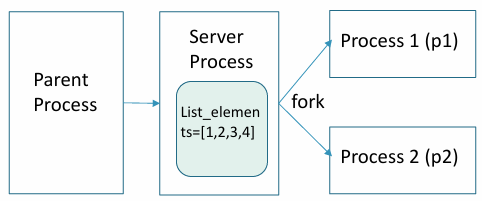
\includegraphics[width=0.45\textwidth]{figuresP/lesson_parallel_2B_pag_13}
\end{center}

\begin{Verbatim}[label=\makebox{\url{https://github.com/lucabaldini/cmepda/tree/master/slides/latex/snippets/multiprocessing_manager.py}},commandchars=\\\{\}]
\PY{k}{import} \PY{n+nn}{multiprocessing}

\PY{k}{def} \PY{n+nf}{add\PYZus{}element}\PY{p}{(}\PY{n}{record}\PY{p}{,}\PY{n}{records}\PY{p}{)}\PY{p}{:}
    \PY{n}{records}\PY{o}{.}\PY{n}{append}\PY{p}{(}\PY{n}{record}\PY{p}{)}
    \PY{n+nb}{print}\PY{p}{(}\PY{l+s+s2}{\PYZdq{}}\PY{l+s+s2}{New element added to records list}\PY{l+s+s2}{\PYZdq{}}\PY{p}{)}

\PY{k}{def} \PY{n+nf}{sum\PYZus{}elements}\PY{p}{(}\PY{n}{records}\PY{p}{)}\PY{p}{:}
    \PY{n}{summ}\PY{o}{=}\PY{n+nb}{sum}\PY{p}{(}\PY{n}{records}\PY{p}{)}
    \PY{n+nb}{print}\PY{p}{(}\PY{l+s+s2}{\PYZdq{}}\PY{l+s+s2}{New sum is: }\PY{l+s+s2}{\PYZdq{}}\PY{o}{+}\PY{n+nb}{str}\PY{p}{(}\PY{n}{summ}\PY{p}{)}\PY{p}{)}

\PY{c+c1}{\#MAIN}
\PY{k}{if} \PY{n}{\PYZus{}\PYZus{}name\PYZus{}\PYZus{}} \PY{o}{==} \PY{l+s+s1}{\PYZsq{}}\PY{l+s+s1}{\PYZus{}\PYZus{}main\PYZus{}\PYZus{}}\PY{l+s+s1}{\PYZsq{}}\PY{p}{:}
    \PY{c+c1}{\# Defining the manager (or server process)}
    \PY{k}{with} \PY{n}{multiprocessing}\PY{o}{.}\PY{n}{Manager}\PY{p}{(}\PY{p}{)} \PY{k}{as} \PY{n}{manager}\PY{p}{:}
        \PY{n}{list\PYZus{}elements}\PY{o}{=}\PY{p}{[}\PY{l+m+mi}{1}\PY{p}{,}\PY{l+m+mi}{2}\PY{p}{,}\PY{l+m+mi}{3}\PY{p}{,}\PY{l+m+mi}{4}\PY{p}{]}
        \PY{c+c1}{\# Here the list becomes \PYZdq{}usable\PYZdq{} for all the processes managed by the manager}
        \PY{n}{records}\PY{o}{=}\PY{n}{manager}\PY{o}{.}\PY{n}{list}\PY{p}{(}\PY{n}{list\PYZus{}elements}\PY{p}{)}
        \PY{n}{new\PYZus{}element}\PY{o}{=}\PY{l+m+mi}{5}

        \PY{n+nb}{print}\PY{p}{(}\PY{l+s+s2}{\PYZdq{}}\PY{l+s+s2}{Old sum is: }\PY{l+s+s2}{\PYZdq{}}\PY{o}{+}\PY{n+nb}{str}\PY{p}{(}\PY{n+nb}{sum}\PY{p}{(}\PY{n}{list\PYZus{}elements}\PY{p}{)}\PY{p}{)}\PY{p}{)}
        \PY{c+c1}{\# Creating new processes}
        \PY{n}{p1} \PY{o}{=} \PY{n}{multiprocessing}\PY{o}{.}\PY{n}{Process}\PY{p}{(}\PY{n}{target}\PY{o}{=}\PY{n}{add\PYZus{}element}\PY{p}{,} \PY{n}{args}\PY{o}{=}\PY{p}{(}\PY{n}{new\PYZus{}element}\PY{p}{,}\PY{n}{records}\PY{p}{)}\PY{p}{)}
        \PY{n}{p2} \PY{o}{=} \PY{n}{multiprocessing}\PY{o}{.}\PY{n}{Process}\PY{p}{(}\PY{n}{target}\PY{o}{=}\PY{n}{sum\PYZus{}elements}\PY{p}{,} \PY{n}{args}\PY{o}{=}\PY{p}{(}\PY{n}{records}\PY{p}{,}\PY{p}{)}\PY{p}{)}

        \PY{c+c1}{\# Running process p1 to insert new element}
        \PY{n}{p1}\PY{o}{.}\PY{n}{start}\PY{p}{(}\PY{p}{)}
        \PY{n}{p1}\PY{o}{.}\PY{n}{join}\PY{p}{(}\PY{p}{)}

        \PY{c+c1}{\# Running process p2 to sum list elements}
        \PY{n}{p2}\PY{o}{.}\PY{n}{start}\PY{p}{(}\PY{p}{)}
        \PY{n}{p2}\PY{o}{.}\PY{n}{join}\PY{p}{(}\PY{p}{)}

[Output]
Old sum is: 10
New element added to records list
New sum is: 15
\end{Verbatim}

\subsubsection{- Queue}

A simple way to communicate between processes with \texttt{multiprocessing} is to use a \textbf{queue} to pass messages back and forth. Any Python object can pass through a \texttt{multiprocessing.Queue()} object. Processes called \textit{producers} write something in the queue (\texttt{Queue.put()}), while the \textit{consumers} are the ones that read data from it. Here's an example:

\begin{center}
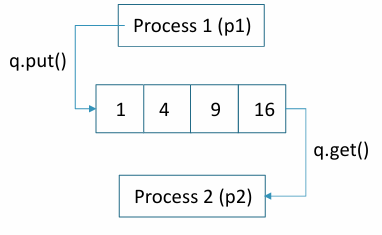
\includegraphics[width=0.4\textwidth]{figuresP/lesson_parallel_2B_pag_14}
\end{center}

\begin{Verbatim}[label=\makebox{\url{https://github.com/lucabaldini/cmepda/tree/master/slides/latex/snippets/multiprocessing_queue_passing.py}},commandchars=\\\{\}]
\PY{k}{import} \PY{n+nn}{multiprocessing}

\PY{k}{def} \PY{n+nf}{square\_list}\PY{p}{(}\PY{n}{mylist}\PY{p}{,} \PY{n}{q}\PY{p}{)}\PY{p}{:}
    \PY{c+c1}{\# Append squares of mylist to queue}
    \PY{k}{for} \PY{n}{num} \PY{k}{in} \PY{n}{mylist}\PY{p}{:}
        \PY{n}{q}\PY{o}{.}\PY{n}{put}\PY{p}{(}\PY{n}{num} \PY{o}{*} \PY{n}{num}\PY{p}{)}

\PY{k}{def} \PY{n+nf}{print\_queue}\PY{p}{(}\PY{n}{q}\PY{p}{)}\PY{p}{:}
    \PY{c+c1}{\# Function to print the elements in the Queue and empty it}
    \PY{n+nb}{print}\PY{p}{(}\PY{l+s+s2}{\PYZdq{}}\PY{l+s+s2}{Queue elements:}\PY{l+s+s2}{\PYZdq{}}\PY{p}{)}
    \PY{k}{while} \PY{o}{not} \PY{n}{q}\PY{o}{.}\PY{n}{empty}\PY{p}{(}\PY{p}{)}\PY{p}{:}
        \PY{n+nb}{print}\PY{p}{(}\PY{n}{q}\PY{o}{.}\PY{n}{get}\PY{p}{(}\PY{p}{)}\PY{p}{)}
    \PY{n+nb}{print}\PY{p}{(}\PY{l+s+s2}{\PYZdq{}}\PY{l+s+s2}{Queue is now empty!}\PY{l+s+s2}{\PYZdq{}}\PY{p}{)}

\PY{c+c1}{\#MAIN}
\PY{k}{if} \PY{n}{\_\_name\_\_}\PY{o}{==}\PY{l+s+s2}{\PYZdq{}}\PY{l+s+s2}{\_\_main\_\_}\PY{l+s+s2}{\PYZdq{}}\PY{p}{:}
    \PY{c+c1}{\# Input list}
    \PY{n}{mylist} \PY{o}{=} \PY{p}{[}\PY{l+m+mi}{1}\PY{p}{,}\PY{l+m+mi}{2}\PY{p}{,}\PY{l+m+mi}{3}\PY{p}{,}\PY{l+m+mi}{4}\PY{p}{]}
    \PY{c+c1}{\# Creating multiprocessing.Queue}
    \PY{n}{q} \PY{o}{=} \PY{n}{multiprocessing}\PY{o}{.}\PY{n}{Queue}\PY{p}{(}\PY{p}{)}

    \PY{c+c1}{\# Creating new processes}
    \PY{n}{p1} \PY{o}{=} \PY{n}{multiprocessing}\PY{o}{.}\PY{n}{Process}\PY{p}{(}\PY{n}{target}\PY{o}{=}\PY{n}{square\_list}\PY{p}{,} \PY{n}{args}\PY{o}{=}\PY{p}{(}\PY{n}{mylist}\PY{p}{,} \PY{n}{q}\PY{p}{)}\PY{p}{)}
    \PY{n}{p2} \PY{o}{=} \PY{n}{multiprocessing}\PY{o}{.}\PY{n}{Process}\PY{p}{(}\PY{n}{target}\PY{o}{=}\PY{n}{print\_queue}\PY{p}{,} \PY{n}{args}\PY{o}{=}\PY{p}{(}\PY{n}{q}\PY{p}{,}\PY{p}{)}\PY{p}{)}

    \PY{c+c1}{\# Running process p1 to square list}
    \PY{n}{p1}\PY{o}{.}\PY{n}{start}\PY{p}{(}\PY{p}{)}
    \PY{n}{p1}\PY{o}{.}\PY{n}{join}\PY{p}{(}\PY{p}{)}
    \PY{c+c1}{\# Running process p2 to get queue elements}
    \PY{n}{p2}\PY{o}{.}\PY{n}{start}\PY{p}{(}\PY{p}{)}
    \PY{n}{p2}\PY{o}{.}\PY{n}{join}\PY{p}{(}\PY{p}{)}

[Output]
Queue elements:
1
4
9
16
Queue is now empty!
\end{Verbatim}

\subsubsection{- Pipe}

A faster way to do practically the same thing is using a \textbf{pipe}. A pipe can have only two endpoints, hence it is preferred over a queue when only two-way communication is required. A queue is slower and it is built on top of a pipe. The \texttt{multiprocessing} module provides the \texttt{multiprocessing.Pipe()} class, which returns a pair of connection objects connected by a pipe (the two ends of the pipe itself). Each connection object has \texttt{send()} and \texttt{recv()} methods (among others), as shown in the following example.

\begin{center}
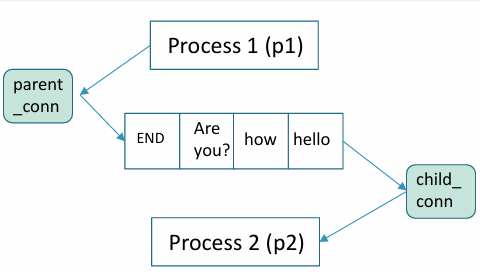
\includegraphics[width=0.4\textwidth]{figuresP/lesson_parallel_2B_pag_15}
\end{center}

\begin{Verbatim}[label=\makebox{\url{https://github.com/lucabaldini/cmepda/tree/master/slides/latex/snippets/multiprocessing_pipe.py}},commandchars=\\\{\}]
\PY{k}{import} \PY{n+nn}{multiprocessing}
\PY{k}{import} \PY{n+nn}{time}

\PY{k}{def} \PY{n+nf}{sender}\PY{p}{(}\PY{n}{conn}\PY{p}{,} \PY{n}{msgs}\PY{p}{)}\PY{p}{:}
    \PY{c+c1}{\# Function for the sender}
    \PY{k}{for} \PY{n}{msg} \PY{k}{in} \PY{n}{msgs}\PY{p}{:}
        \PY{n}{time}\PY{o}{.}\PY{n}{sleep}\PY{p}{(}\PY{l+m+mi}{1}\PY{p}{)}
        \PY{n}{conn}\PY{o}{.}\PY{n}{send}\PY{p}{(}\PY{n}{msg}\PY{p}{)}
        \PY{n+nb}{print}\PY{p}{(}\PY{l+s+s2}{\PYZdq{}}\PY{l+s+s2}{Sent the message: }\PY{l+s+s2}{\PYZdq{}}\PY{o}{+}\PY{n+nb}{str}\PY{p}{(}\PY{n}{msg}\PY{p}{)}\PY{p}{)}

    \PY{n}{conn}\PY{o}{.}\PY{n}{close}\PY{p}{(}\PY{p}{)}

\PY{k}{def} \PY{n+nf}{receiver}\PY{p}{(}\PY{n}{conn}\PY{p}{)}\PY{p}{:}
    \PY{c+c1}{\# Function for the receiver}
    \PY{n}{time}\PY{o}{.}\PY{n}{sleep}\PY{p}{(}\PY{l+m+mi}{2}\PY{p}{)}
    \PY{k}{while} \PY{l+m+mi}{1}\PY{p}{:}
        \PY{n}{msg} \PY{o}{=} \PY{n}{conn}\PY{o}{.}\PY{n}{recv}\PY{p}{(}\PY{p}{)}

        \PY{k}{if} \PY{n}{msg} \PY{o}{==} \PY{l+s+s2}{\PYZdq{}}\PY{l+s+s2}{END}\PY{l+s+s2}{\PYZdq{}}\PY{p}{:}
            \PY{k}{break}
        \PY{n+nb}{print}\PY{p}{(}\PY{l+s+s2}{\PYZdq{}}\PY{l+s+s2}{Received the message: }\PY{l+s+s2}{\PYZdq{}}\PY{o}{+}\PY{n+nb}{str}\PY{p}{(}\PY{n}{msg}\PY{p}{)}\PY{p}{)}

\PY{c+c1}{\#MAIN}
\PY{k}{if} \PY{n}{\_\_name\_\_}\PY{o}{==}\PY{l+s+s2}{\PYZdq{}}\PY{l+s+s2}{\_\_main\_\_}\PY{l+s+s2}{\PYZdq{}}\PY{p}{:}
    \PY{c+c1}{\# Messages to be sent}
    \PY{n}{msgs} \PY{o}{=} \PY{p}{[}\PY{l+s+s2}{\PYZdq{}}\PY{l+s+s2}{hello,}\PY{l+s+s2}{\PYZdq{}}\PY{p}{,} \PY{l+s+s2}{\PYZdq{}}\PY{l+s+s2}{how}\PY{l+s+s2}{\PYZdq{}}\PY{p}{,} \PY{l+s+s2}{\PYZdq{}}\PY{l+s+s2}{are you?}\PY{l+s+s2}{\PYZdq{}}\PY{p}{,} \PY{l+s+s2}{\PYZdq{}}\PY{l+s+s2}{END}\PY{l+s+s2}{\PYZdq{}}\PY{p}{]}
    \PY{c+c1}{\# Creating a pipe}
    \PY{n}{parent\PYZus{}conn}\PY{p}{,} \PY{n}{child\PYZus{}conn} \PY{o}{=} \PY{n}{multiprocessing}\PY{o}{.}\PY{n}{Pipe}\PY{p}{(}\PY{p}{)}

    \PY{c+c1}{\# Creating new processes}
    \PY{n}{p1} \PY{o}{=} \PY{n}{multiprocessing}\PY{o}{.}\PY{n}{Process}\PY{p}{(}\PY{n}{target}\PY{o}{=}\PY{n}{sender}\PY{p}{,} \PY{n}{args}\PY{o}{=}\PY{p}{(}\PY{n}{parent\PYZus{}conn}\PY{p}{,}\PY{n}{msgs}\PY{p}{)}\PY{p}{)}
    \PY{n}{p2} \PY{o}{=} \PY{n}{multiprocessing}\PY{o}{.}\PY{n}{Process}\PY{p}{(}\PY{n}{target}\PY{o}{=}\PY{n}{receiver}\PY{p}{,} \PY{n}{args}\PY{o}{=}\PY{p}{(}\PY{n}{child\PYZus{}conn}\PY{p}{,}\PY{p}{)}\PY{p}{)}

    \PY{c+c1}{\# Running processes}
    \PY{n}{p1}\PY{o}{.}\PY{n}{start}\PY{p}{(}\PY{p}{)}
    \PY{n}{p2}\PY{o}{.}\PY{n}{start}\PY{p}{(}\PY{p}{)}
    \PY{c+c1}{\# Wait until processes finish}
    \PY{n}{p1}\PY{o}{.}\PY{n}{join}\PY{p}{(}\PY{p}{)}
    \PY{n}{p2}\PY{o}{.}\PY{n}{join}\PY{p}{(}\PY{p}{)}

[Output]
Sent the message: hello,
Sent the message: how
Received the message: hello,
Received the message: how
Sent the message: are you?
Received the message: are you?
Sent the message: END
\end{Verbatim}

\subsection{Synchronization for processes: locking in Python}

\textbf{Process synchronization} is defined as a mechanism which ensures that two or more concurrent processes do not simultaneously execute some particular program segment known as \textbf{critical section}. A \textbf{race condition} occurs when two or more processes can access shared data and they try to change it at the same time. As a result, the values of variables may be unpredictable and vary depending on the timings of context switches of the processes.

Take a look at the following example. Here synchronization is not implemented and the results vary each time. It's a disaster!

\begin{Verbatim}[label=\makebox{\url{https://github.com/lucabaldini/cmepda/tree/master/slides/latex/snippets/synchro1.py}},commandchars=\\\{\}]
\PY{k}{import} \PY{n+nn}{multiprocessing}

\PY{k}{def} \PY{n+nf}{withdraw}\PY{p}{(}\PY{n}{balance}\PY{p}{)}\PY{p}{:}
    \PY{c+c1}{\# Function to withdraw from account}
    \PY{k}{for} \PY{n}{x} \PY{k}{in} \PY{n+nb}{range}\PY{p}{(}\PY{l+m+mi}{10000}\PY{p}{)}\PY{p}{:}
            \PY{n}{balance}\PY{o}{.}\PY{n}{value} \PY{o}{=} \PY{n}{balance}\PY{o}{.}\PY{n}{value}\PY{o}{\PYZhy{}}\PY{l+m+mi}{1}

\PY{k}{def} \PY{n+nf}{deposit}\PY{p}{(}\PY{n}{balance}\PY{p}{)}\PY{p}{:}
    \PY{c+c1}{\# Function to deposit in the account}
    \PY{k}{for} \PY{n}{x} \PY{k}{in} \PY{n+nb}{range}\PY{p}{(}\PY{l+m+mi}{10000}\PY{p}{)}\PY{p}{:}
        \PY{n}{balance}\PY{o}{.}\PY{n}{value} \PY{o}{=} \PY{n}{balance}\PY{o}{.}\PY{n}{value} \PY{o}{+} \PY{l+m+mi}{1}

\PY{k}{def} \PY{n+nf}{perform\PYZus{}transactions}\PY{p}{(}\PY{p}{)}\PY{p}{:}
    \PY{c+c1}{\# Initial balance (in shared memory) = 100\PYZdl{}}
    \PY{n}{balance} \PY{o}{=} \PY{n}{multiprocessing}\PY{o}{.}\PY{n}{Value}\PY{p}{(}\PY{l+s+s1}{\PYZsq{}}\PY{l+s+s1}{i}\PY{l+s+s1}{\PYZsq{}}\PY{p}{,} \PY{l+m+mi}{100}\PY{p}{)}
    \PY{c+c1}{\# Creating new processes}
    \PY{n}{p1} \PY{o}{=} \PY{n}{multiprocessing}\PY{o}{.}\PY{n}{Process}\PY{p}{(}\PY{n}{target}\PY{o}{=}\PY{n}{withdraw}\PY{p}{,} \PY{n}{args}\PY{o}{=}\PY{p}{(}\PY{n}{balance}\PY{p}{,}\PY{p}{)}\PY{p}{)}
    \PY{n}{p2} \PY{o}{=} \PY{n}{multiprocessing}\PY{o}{.}\PY{n}{Process}\PY{p}{(}\PY{n}{target}\PY{o}{=}\PY{n}{deposit}\PY{p}{,} \PY{n}{args}\PY{o}{=}\PY{p}{(}\PY{n}{balance}\PY{p}{,}\PY{p}{)}\PY{p}{)}
    \PY{c+c1}{\# Starting processes}
    \PY{n}{p1}\PY{o}{.}\PY{n}{start}\PY{p}{(}\PY{p}{)}
    \PY{n}{p2}\PY{o}{.}\PY{n}{start}\PY{p}{(}\PY{p}{)}
    \PY{c+c1}{\# Wait until processes are finished}
    \PY{n}{p1}\PY{o}{.}\PY{n}{join}\PY{p}{(}\PY{p}{)}
    \PY{n}{p2}\PY{o}{.}\PY{n}{join}\PY{p}{(}\PY{p}{)}
    \PY{c+c1}{\# Print final balance}
    \PY{n+nb}{print}\PY{p}{(}\PY{l+s+s2}{\PYZdq{}}\PY{l+s+s2}{Final balance = }\PY{l+s+si}{\PYZob{}\PYZcb{}}\PY{l+s+s2}{\PYZdq{}}\PY{o}{.}\PY{n}{format}\PY{p}{(}\PY{n}{balance}\PY{o}{.}\PY{n}{value}\PY{p}{)}\PY{p}{)}

\PY{c+c1}{\#MAIN}
\PY{k}{if} \PY{n}{\_\_name\_\_}\PY{o}{==}\PY{l+s+s2}{\PYZdq{}}\PY{l+s+s2}{\_\_main\_\_}\PY{l+s+s2}{\PYZdq{}}\PY{p}{:}
    \PY{k}{for} \PY{n}{x} \PY{k}{in} \PY{n+nb}{range}\PY{p}{(}\PY{l+m+mi}{10}\PY{p}{)}\PY{p}{:}
        \PY{c+c1}{\# Perform the same transaction process 10 times without syncrhonization}
        \PY{n}{perform\PYZus{}transactions}\PY{p}{(}\PY{p}{)}

[Output]
Final balance = 614
Final balance = -4609
Final balance = -176
Final balance = -1183
Final balance = 1896
Final balance = 138
Final balance = 699
Final balance = 2840
Final balance = -473
Final balance = -2117
\end{Verbatim}

The \texttt{multiprocessing} module provides a \texttt{Lock} class to deal with the race conditions, which is implemented using a Semaphore object provided by the OS, as shown below. As said, a semaphore is a synchronization object that controls access by multiple processes to a common resource in a parallel programming environment. It is simply a value in a designated place in the operating system (or kernel) storage that each process can check and then change. Depending on the value that is found, the process can use the resource or will find that it is already in use and must wait for some time before trying again.  

\begin{Verbatim}[label=\makebox{\url{https://github.com/lucabaldini/cmepda/tree/master/slides/latex/snippets/synchro2.py}},commandchars=\\\{\}]
\PY{k}{import} \PY{n+nn}{multiprocessing}

\PY{k}{def} \PY{n+nf}{withdraw}\PY{p}{(}\PY{n}{balance}\PY{p}{,} \PY{n}{lock}\PY{p}{)}\PY{p}{:}
    \PY{c+c1}{\# Function to withdraw from account}
    \PY{k}{for} \PY{n}{x} \PY{k}{in} \PY{n+nb}{range}\PY{p}{(}\PY{l+m+mi}{10000}\PY{p}{)}\PY{p}{:}
        \PY{c+c1}{\# Implementing a locking mechanism: syncrhonization}
        \PY{n}{lock}\PY{o}{.}\PY{n}{acquire}\PY{p}{(}\PY{p}{)}
        \PY{n}{balance}\PY{o}{.}\PY{n}{value} \PY{o}{=} \PY{n}{balance}\PY{o}{.}\PY{n}{value} \PY{o}{\PYZhy{}} \PY{l+m+mi}{1}
        \PY{n}{lock}\PY{o}{.}\PY{n}{release}\PY{p}{(}\PY{p}{)}

\PY{k}{def} \PY{n+nf}{deposit}\PY{p}{(}\PY{n}{balance}\PY{p}{,} \PY{n}{lock}\PY{p}{)}\PY{p}{:}
    \PY{c+c1}{\# Function to deposit to account}
    \PY{k}{for} \PY{n}{x} \PY{k}{in} \PY{n+nb}{range}\PY{p}{(}\PY{l+m+mi}{10000}\PY{p}{)}\PY{p}{:}
        \PY{c+c1}{\# Implementing a locking mechanism: syncrhonization}
        \PY{n}{lock}\PY{o}{.}\PY{n}{acquire}\PY{p}{(}\PY{p}{)}
        \PY{n}{balance}\PY{o}{.}\PY{n}{value} \PY{o}{=} \PY{n}{balance}\PY{o}{.}\PY{n}{value} \PY{o}{+} \PY{l+m+mi}{1}
        \PY{n}{lock}\PY{o}{.}\PY{n}{release}\PY{p}{(}\PY{p}{)}

\PY{k}{def} \PY{n+nf}{perform\PYZus{}transactions}\PY{p}{(}\PY{p}{)}\PY{p}{:}
    \PY{c+c1}{\# Initial balance (in shared memory)}
    \PY{n}{balance} \PY{o}{=} \PY{n}{multiprocessing}\PY{o}{.}\PY{n}{Value}\PY{p}{(}\PY{l+s+s1}{\PYZsq{}}\PY{l+s+s1}{i}\PY{l+s+s1}{\PYZsq{}}\PY{p}{,} \PY{l+m+mi}{100}\PY{p}{)}
    \PY{c+c1}{\# Creating a lock object}
    \PY{n}{lock} \PY{o}{=} \PY{n}{multiprocessing}\PY{o}{.}\PY{n}{Lock}\PY{p}{(}\PY{p}{)}

    \PY{c+c1}{\# Creating new processes}
    \PY{n}{p1} \PY{o}{=} \PY{n}{multiprocessing}\PY{o}{.}\PY{n}{Process}\PY{p}{(}\PY{n}{target}\PY{o}{=}\PY{n}{withdraw}\PY{p}{,} \PY{n}{args}\PY{o}{=}\PY{p}{(}\PY{n}{balance}\PY{p}{,}\PY{n}{lock}\PY{p}{)}\PY{p}{)}
    \PY{n}{p2} \PY{o}{=} \PY{n}{multiprocessing}\PY{o}{.}\PY{n}{Process}\PY{p}{(}\PY{n}{target}\PY{o}{=}\PY{n}{deposit}\PY{p}{,} \PY{n}{args}\PY{o}{=}\PY{p}{(}\PY{n}{balance}\PY{p}{,}\PY{n}{lock}\PY{p}{)}\PY{p}{)}
    \PY{c+c1}{\# Starting processes}
    \PY{n}{p1}\PY{o}{.}\PY{n}{start}\PY{p}{(}\PY{p}{)}
    \PY{n}{p2}\PY{o}{.}\PY{n}{start}\PY{p}{(}\PY{p}{)}
    \PY{c+c1}{\# Wait until processes are finished}
    \PY{n}{p1}\PY{o}{.}\PY{n}{join}\PY{p}{(}\PY{p}{)}
    \PY{n}{p2}\PY{o}{.}\PY{n}{join}\PY{p}{(}\PY{p}{)}

    \PY{c+c1}{\# Print final balance}
    \PY{n+nb}{print}\PY{p}{(}\PY{l+s+s2}{\PYZdq{}}\PY{l+s+s2}{Final balance = }\PY{l+s+s2}{\PYZdq{}}\PY{o}{+}\PY{n+nb}{str}\PY{p}{(}\PY{n}{balance}\PY{o}{.}\PY{n}{value}\PY{p}{)}\PY{p}{)}

\PY{c+c1}{\#MAIN}
\PY{k}{if} \PY{n}{\_\_name\_\_}\PY{o}{==}\PY{l+s+s2}{\PYZdq{}}\PY{l+s+s2}{\_\_main\_\_}\PY{l+s+s2}{\PYZdq{}}\PY{p}{:}
    \PY{k}{for} \PY{n}{x} \PY{k}{in} \PY{n+nb}{range}\PY{p}{(}\PY{l+m+mi}{10}\PY{p}{)}\PY{p}{:}
        \PY{c+c1}{\# Perform the same transaction process 10 times with syncrhonization}
        \PY{n}{perform\PYZus{}transactions}\PY{p}{(}\PY{p}{)}

[Output]
Final balance = 100
Final balance = 100
Final balance = 100
Final balance = 100
Final balance = 100
Final balance = 100
Final balance = 100
Final balance = 100
Final balance = 100
Final balance = 100
\end{Verbatim}

\subsection{Threading in Python} 


\begin{figure}[H]
\begin{minipage}{0.55\textwidth}
As said, multiple threads (which share the same global variables stored in the heap) can exist within one process, and each one of them contains its own register set and local variables (stored in the stack), as represented in figure.

\subsubsection{- The \texttt{threading} module}

Here's a simple example on how to define multiple threads using the \texttt{Thread} object in the \texttt{threading} module. Note that the syntax is very much similar to the \texttt{multiprocessing} module. First of all note that the PID of the process is the same for both threads, as expected. The following piece of code gives the impression that the threads \texttt{t1} and \texttt{t2} are running in parallel, but due to the GIL that's not the case. 

\end{minipage}\hfill
\begin{minipage}[c]{0.38\textwidth}
\centering
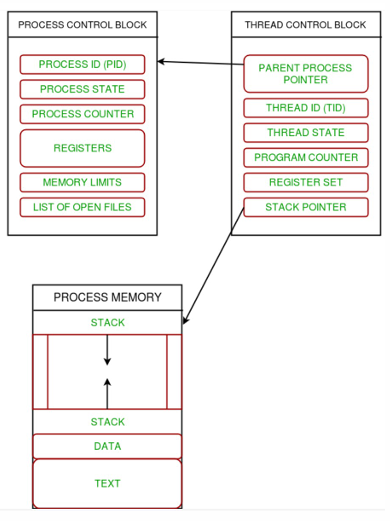
\includegraphics[width=\textwidth]{figuresP/lesson_parallel_2B_pag_18}
\end{minipage}
\end{figure}

%\begin{center}
%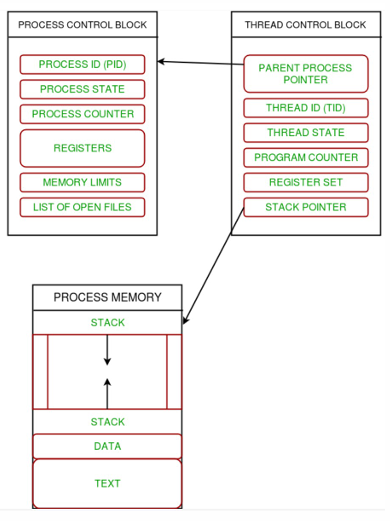
\includegraphics[width=0.3\textwidth]{figuresP/lesson_parallel_2B_pag_18}
%\end{center}

\begin{Verbatim}[label=\makebox{\url{https://github.com/lucabaldini/cmepda/tree/master/slides/latex/snippets/threading_basic.py}},commandchars=\\\{\}]
\PY{k}{import} \PY{n+nn}{threading}
\PY{k}{import} \PY{n+nn}{os}

\PY{k}{def} \PY{n+nf}{task1}\PY{p}{(}\PY{p}{)}\PY{p}{:}
        \PY{n+nb}{print}\PY{p}{(}\PY{l+s+s2}{\PYZdq{}}\PY{l+s+s2}{Task 1 assigned to thread: }\PY{l+s+s2}{\PYZdq{}}\PY{o}{+}\PY{n}{threading}\PY{o}{.}\PY{n}{current\PYZus{}thread}\PY{p}{(}\PY{p}{)}\PY{o}{.}\PY{n}{name}\PY{p}{)}
        \PY{n+nb}{print}\PY{p}{(}\PY{l+s+s2}{\PYZdq{}}\PY{l+s+s2}{ID of process running task 1: }\PY{l+s+s2}{\PYZdq{}}\PY{o}{+}\PY{n+nb}{str}\PY{p}{(}\PY{n}{os}\PY{o}{.}\PY{n}{getpid}\PY{p}{(}\PY{p}{)}\PY{p}{)}\PY{p}{)}
\PY{k}{def} \PY{n+nf}{task2}\PY{p}{(}\PY{p}{)}\PY{p}{:}
        \PY{n+nb}{print}\PY{p}{(}\PY{l+s+s2}{\PYZdq{}}\PY{l+s+s2}{Task 2 assigned to thread: }\PY{l+s+s2}{\PYZdq{}}\PY{o}{+}\PY{n}{threading}\PY{o}{.}\PY{n}{current\PYZus{}thread}\PY{p}{(}\PY{p}{)}\PY{o}{.}\PY{n}{name}\PY{p}{)}
        \PY{n+nb}{print}\PY{p}{(}\PY{l+s+s2}{\PYZdq{}}\PY{l+s+s2}{ID of process running task 2: }\PY{l+s+s2}{\PYZdq{}}\PY{o}{+}\PY{n+nb}{str}\PY{p}{(}\PY{n}{os}\PY{o}{.}\PY{n}{getpid}\PY{p}{(}\PY{p}{)}\PY{p}{)}\PY{p}{)}
\PY{c+c1}{\#MAIN}
\PY{k}{if} \PY{n}{\_\_name\_\_}\PY{o}{==}\PY{l+s+s2}{\PYZdq{}}\PY{l+s+s2}{\_\_main\_\_}\PY{l+s+s2}{\PYZdq{}}\PY{p}{:}
        \PY{c+c1}{\# Print ID of current process}
        \PY{n+nb}{print}\PY{p}{(}\PY{l+s+s2}{\PYZdq{}}\PY{l+s+s2}{ID of process running main program: }\PY{l+s+s2}{\PYZdq{}}\PY{o}{+}\PY{n+nb}{str}\PY{p}{(}\PY{n}{os}\PY{o}{.}\PY{n}{getpid}\PY{p}{(}\PY{p}{)}\PY{p}{)}\PY{p}{)}
        \PY{c+c1}{\# Print name of main thread}
        \PY{n+nb}{print}\PY{p}{(}\PY{l+s+s2}{\PYZdq{}}\PY{l+s+s2}{Main thread name: }\PY{l+s+s2}{\PYZdq{}}\PY{o}{+}\PY{n}{threading}\PY{o}{.}\PY{n}{main\PYZus{}thread}\PY{p}{(}\PY{p}{)}\PY{o}{.}\PY{n}{name}\PY{p}{)}

        \PY{c+c1}{\# Creating threads}
        \PY{n}{t1} \PY{o}{=} \PY{n}{threading}\PY{o}{.}\PY{n}{Thread}\PY{p}{(}\PY{n}{target}\PY{o}{=}\PY{n}{task1}\PY{p}{,} \PY{n}{name}\PY{o}{=}\PY{l+s+s1}{\PYZsq{}}\PY{l+s+s1}{t1}\PY{l+s+s1}{\PYZsq{}}\PY{p}{)}
        \PY{n}{t2} \PY{o}{=} \PY{n}{threading}\PY{o}{.}\PY{n}{Thread}\PY{p}{(}\PY{n}{target}\PY{o}{=}\PY{n}{task2}\PY{p}{,} \PY{n}{name}\PY{o}{=}\PY{l+s+s1}{\PYZsq{}}\PY{l+s+s1}{t2}\PY{l+s+s1}{\PYZsq{}}\PY{p}{)}
        \PY{c+c1}{\# Starting threads}
        \PY{n}{t1}\PY{o}{.}\PY{n}{start}\PY{p}{(}\PY{p}{)}
        \PY{n}{t2}\PY{o}{.}\PY{n}{start}\PY{p}{(}\PY{p}{)}
        \PY{c+c1}{\# Wait until all threads finish}
        \PY{n}{t1}\PY{o}{.}\PY{n}{join}\PY{p}{(}\PY{p}{)}
        \PY{n}{t2}\PY{o}{.}\PY{n}{join}\PY{p}{(}\PY{p}{)}

[Output]
ID of process running main program: 54321
Main thread name: MainThread
Task 1 assigned to thread: t1
ID of process running task 1: 54321
Task 2 assigned to thread: t2
ID of process running task 2: 54321
\end{Verbatim}

The following example shows how the GIL intervenes during code execution. Even though you should easily be able to see how a race condition should happen at runtime, the result is actually correct. That's the GIL's work: different threads are always executed at different times. 

\begin{Verbatim}[label=\makebox{\url{https://github.com/lucabaldini/cmepda/tree/master/slides/latex/snippets/threading_race_condition.py}},commandchars=\\\{\}]
\PY{k}{import} \PY{n+nn}{threading}

\PY{c+c1}{\# Global variable x}
\PY{n}{x} \PY{o}{=} \PY{l+m+mi}{0}

\PY{k}{def} \PY{n+nf}{increment}\PY{p}{(}\PY{p}{)}\PY{p}{:}
    \PY{k}{global} \PY{n}{x}
    \PY{n}{x} \PY{o}{+}\PY{o}{=} \PY{l+m+mi}{1}

\PY{k}{def} \PY{n+nf}{thread\_task}\PY{p}{(}\PY{p}{)}\PY{p}{:}
    \PY{k}{for} \PY{n}{\_} \PY{k}{in} \PY{n+nb}{range}\PY{p}{(}\PY{l+m+mi}{100000}\PY{p}{)}\PY{p}{:}
        \PY{n}{increment}\PY{p}{(}\PY{p}{)}

\PY{k}{def} \PY{n+nf}{main\_task}\PY{p}{(}\PY{p}{)}\PY{p}{:}
    \PY{k}{global} \PY{n}{x}
    \PY{c+c1}{\# Setting global variable x as 0}
    \PY{n}{x} \PY{o}{=} \PY{l+m+mi}{0}
    \PY{c+c1}{\# Creating threads}
    \PY{n}{t1} \PY{o}{=} \PY{n}{threading}\PY{o}{.}\PY{n}{Thread}\PY{p}{(}\PY{n}{target}\PY{o}{=}\PY{n}{thread\_task}\PY{p}{)}
    \PY{n}{t2} \PY{o}{=} \PY{n}{threading}\PY{o}{.}\PY{n}{Thread}\PY{p}{(}\PY{n}{target}\PY{o}{=}\PY{n}{thread\_task}\PY{p}{)}

    \PY{c+c1}{\# Start threads}
    \PY{n}{t1}\PY{o}{.}\PY{n}{start}\PY{p}{(}\PY{p}{)}
    \PY{n}{t2}\PY{o}{.}\PY{n}{start}\PY{p}{(}\PY{p}{)}
    \PY{c+c1}{\# Wait until threads finish their job}
    \PY{n}{t1}\PY{o}{.}\PY{n}{join}\PY{p}{(}\PY{p}{)}
    \PY{n}{t2}\PY{o}{.}\PY{n}{join}\PY{p}{(}\PY{p}{)}

\PY{c+c1}{\#MAIN}
\PY{k}{for} \PY{n}{i} \PY{k}{in} \PY{n+nb}{range}\PY{p}{(}\PY{l+m+mi}{10}\PY{p}{)}\PY{p}{:}
    \PY{n}{main\_task}\PY{p}{(}\PY{p}{)}
    \PY{n+nb}{print}\PY{p}{(}\PY{l+s+s2}{\PYZdq{}}\PY{l+s+s2}{Iteration }\PY{l+s+si}{\PYZob{}0\PYZcb{}}\PY{l+s+s2}{: x = }\PY{l+s+si}{\PYZob{}1\PYZcb{}}\PY{l+s+s2}{\PYZdq{}}\PY{o}{.}\PY{n}{format}\PY{p}{(}\PY{n}{i}\PY{p}{,}\PY{n}{x}\PY{p}{)}\PY{p}{)}

[Output]
Iteration 0: x = 200000
Iteration 1: x = 200000
Iteration 2: x = 200000
Iteration 3: x = 200000
Iteration 4: x = 200000
Iteration 5: x = 200000
Iteration 6: x = 200000
Iteration 7: x = 200000
Iteration 8: x = 200000
Iteration 9: x = 200000
\end{Verbatim}

However, it can be useful to implement a locking mechanism while using threading too. 

The GIL solves the problem of race conditions, but there may be some instances when you need a certain thread to run instead of another, even though they are acting on different data (e.g. one thread modifies an image, the other saves it in a folder: you need the first thread to finish before the second one does its job). 

Here's how you can implement synchronization using the \texttt{threading} module (the syntax is exactly the same as before):

\input{pygments/thread2b}

For further information on the \texttt{multiprocessing} and \texttt{threading} modules, take a look at the documentation: \\ - \texttt{multiprocessing}: \url{https://docs.python.org/3/library/multiprocessing.html}
\\ - \texttt{threading}: \url{https://docs.python.org/3/library/threading.html}.

\subsection{Comparison between threads and processes in Python}\label{sec:thread_process}

Lastly, we want to show the fundamental differences between code that utilizes threads and code that uses processes using a more complex example.

We want to write a program to factorize a list of 300 odd numbers between 1'000'000'001 and 1'000'000'597 and we want to measure the time needed to finish this operation using serial code, then 2, 4 or 8 threads and lastly 2, 4 or 8 processes. You can find the full code in Appendix \ref{app:final_example} and you can try to write it yourself. \\
Here's a graph with the result:

\begin{center}
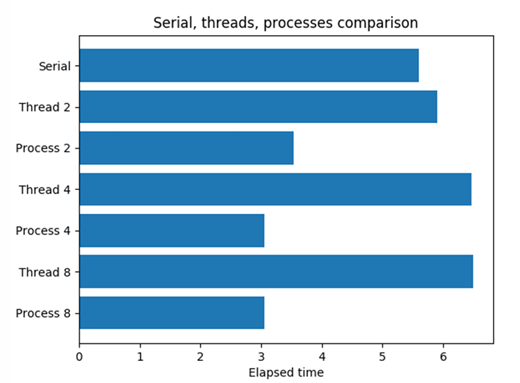
\includegraphics[width=0.6\textwidth]{figuresP/process_thread_comparison.png}
\end{center}

As you can see, the elapsed time with threads is always higher than the one obtained with serial execution. That is due to the GIL. With 2 processes we get a good speed-up, even though the elapsed time is not exactly halved due to the time needed by the OS to "organize" the execution. Moreover, note that with 4 processes we have already reached a saturation point due to Amdahl's law.

With that in mind, an important question is raised: why should I use threads? First of all, in case of I/O operations the GIL releases the lock (as previously said), so if your program needs to rapidly exchange large amounts of data, threads might be the way to go. More importantly (at least for calculus applications), if some of your functions are written in external C code, the GIL mechanism is bypassed and your threads will really be executed in parallel.

Here's another short recap:

\begin{center}
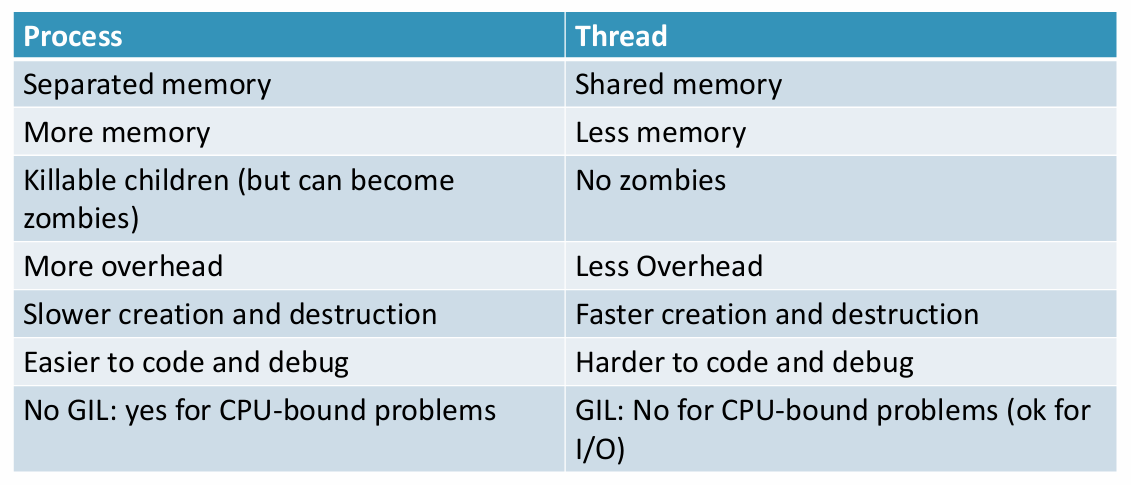
\includegraphics[width=0.7\textwidth]{figuresP/lesson_parallel_2B_pag_27}
\end{center}

A final thought for you: Python is really easy to use and understand, but these last sections should have shown you that it is not very efficient for parallelism. Fortran, C, C++ are better suited for that.

\underline{Final assignment}: Calculate for each number in a list the sum of all primes which are smaller than the given number. It should output the pairs [\texttt{n}, \texttt{sum\_primes(n)}] sorted by \texttt{n}. Example: If the input list is [10, 20], the expected output should be [[10, 17], [20, 77]]. Please use the \texttt{multiprocessing} module and compare the result (in terms of execution time) with the serial version of your code. Try to do the same with the \texttt{threading} module. Use big numbers like 2.5 million.